\documentclass[conference]{IEEEtran}
\usepackage{graphicx}
\usepackage{booktabs}
\usepackage{amsmath}
\usepackage[hidelinks]{hyperref}
\title{Road Accident Severity Prediction with Traffic Volume Ablation and Road Link Holdout Evaluation}
\author{\IEEEauthorblockN{Road Accident Severity Prediction Project Team}}
\begin{document}
\maketitle
\begin{abstract}
We compare multinomial logistic regression, a decision tree and Random Forest for classifying recorded injury crashes as Slight, Serious or Fatal. The study uses prepared 2025 Great Britain STATS19 collision and vehicle records and tests annual average daily flow (AADF) as a traffic-volume proxy. Spatial matching retains 19,397 crashes from 101,525 source collisions. On the fixed crash-level test set of 3,914 collisions, logistic regression achieves macro F1 of 0.4414 without AADF and 0.4350 with AADF, identifying seven of 49 fatal crashes in either configuration. A second experiment separates entire count-point road links between training, validation and test. On its 3,862 test collisions, logistic regression achieves 0.4400 without AADF and 0.4337 with AADF. The separately tuned forest gains slightly from AADF on the link holdout. These results support evaluating traffic features and partition assumptions explicitly, rather than treating traffic volume as an automatic improvement or overall accuracy as evidence of reliable fatal-crash detection.
\end{abstract}
\begin{IEEEkeywords}
crash severity, class imbalance, logistic regression, Random Forest, traffic volume, grouped evaluation
\end{IEEEkeywords}

\section{Introduction}
A severity classifier estimates an outcome conditional on an injury crash having occurred. This differs from forecasting crash occurrence, which would require observations of both crash and non-crash exposure. We study the former task, using the published Slight, Serious and Fatal labels. Slight corresponds to the project's minor-severity category. Reliable comparison requires separating common-class accuracy from performance on rare fatal events.

The requested predictor groups are road type, weather, time, traffic density, vehicle type, speed limit and road surface. The source data do not contain a direct measurement of traffic density at the crash time. We therefore evaluate AADF, a road-link traffic-volume measure, and keep its interpretation distinct from instantaneous density. Our contributions are a reproducible three-model comparison, a controlled AADF ablation on shared test rows, an additional road-link holdout, and exported prediction pipelines with input validation.

\section{Related Work}
Chen and Chen compare logistic regression, classification trees and Random Forest, emphasizing that feature choice affects accuracy, sensitivity and specificity \cite{chen}. Their binary target and Taiwan setting differ from our three-class British crash experiment. The comparison motivates retaining a linear baseline alongside tree methods; it does not establish that one family must win on every dataset.

Fiorentini and Losa investigate majority undersampling and minority-class performance \cite{fiorentini}. Their work supports measuring the effect of imbalance handling beyond overall accuracy. We use training weights and validation-selected decision multipliers without introducing resampled observations into the test set. Kim et al. examine both class imbalance and the ordered nature of severity for older drivers \cite{kim}. Their findings motivate an ordinal-model extension, although our implemented classifiers treat the three labels nominally.

Obasi and Benson compare several learners on earlier UK crash data \cite{obasi}. Their different years and predictors prevent direct numerical comparison with our results. Kuo et al. study resampling and feature-selection order on a small autonomous-vehicle dataset \cite{kuo}. Their setting highlights the need to inspect preprocessing order and sample size. Neither these studies nor our experiments justify transferring performance estimates to a new country without validation.

\section{Data and Feature Construction}
\subsection{Collision and vehicle records}
The supplied 2025 collision file contains 101,525 injury crashes and the vehicle file contains 183,948 records. Source labels comprise 74,881 Slight, 25,191 Serious and 1,453 Fatal collisions. We join tables by collision index, retain one row per collision and aggregate vehicle types into binary involvement flags. A collision involving both a car and a bicycle retains both flags. Missing vehicle types and the explicit unknown-type code have distinct indicators.

Road, weather and surface codes are categorical. Missing surface values retain a separate imputed category. The pipeline one-hot encodes categorical predictors, imputes numeric values using development data at the appropriate fitting stage, and represents clock time cyclically:
\begin{equation}
 t_s=\sin(2\pi m/1440),\quad t_c=\cos(2\pi m/1440),
\end{equation}
where $m$ is minutes since midnight. This keeps times on either side of midnight close in feature space. Logistic regression scales numeric features. Speed is the posted speed limit in miles per hour, not measured vehicle speed. Collision IDs, injury counts, label-derived variables and partition assignments are excluded from predictors.

\subsection{Traffic-volume matching}
We use DfT traffic-count records, count points and major-road geometries \cite{dfttraffic}. A candidate road link must have the same normalized road number, lie within 50 m in British National Grid coordinates, and be more than 10 m closer than the next eligible count-point link. Competing links are searched beyond the main cutoff so that a nearby alternative can invalidate an ambiguous match. Geometry fragments sharing a count-point ID are treated as the same link.

Matching retains 19,397 collisions across 7,778 count-point links. DfT labels 5,872 matched traffic values Counted and 13,525 Estimated. The resulting coverage is 19.1\% of source collisions, so the traffic experiment describes this selected major-road subset. AADF represents typical motor vehicles per day; it cannot establish traffic conditions at the individual crash time. The underlying safety data and definitions are published by DfT \cite{dftsafety}.

\section{Experimental Design}
\subsection{Fixed crash-level split}
The full prepared collision table uses stratified training, validation and test partitions with seed 42. Matched rows inherit these assignments: 12,371 training, 3,112 validation and 3,914 test collisions. The matched test includes 49 fatal collisions. Both feature sets use exactly the same rows, and all six configurations use the same labels and metric definitions.

Logistic regression searches $C\in\{0.1,1,10\}$; the decision tree searches depths 4, 8 and 14 with at least 10 samples per leaf. Both consider unweighted, moderately weighted and balanced training. Decision multipliers for Serious and Fatal are selected on validation rows, with the Slight multiplier fixed at one. Settings selected with AADF are held fixed for the corresponding no-AADF fit. The historical Random Forest uses 150 trees, depth 14, minimum leaf size 10, moderate class weights and previously locked decision multipliers. This protocol compares selected configurations; it does not equalize hyperparameter-search budgets across families.

After selection, a fresh pipeline is fitted on training plus validation. Let $p_c(x)$ be a raw model score and $w_c$ the saved class multiplier. The deployed rule is
\begin{equation}
 \hat{y}=\operatorname*{arg\,max}_{c} w_c p_c(x).
\end{equation}
Adjusted scores are decision quantities, not calibrated probabilities. Reported raw scores can rank classes differently from the final weighted decision.

\subsection{Road-link holdout}
A second experiment uses GroupShuffleSplit with seed 42: 20\% of count-point links form test, followed by 20\% of development links for validation. The resulting partitions contain 4,977 training links, 1,245 validation links and 1,556 test links; no link appears in two partitions. Crash counts are 12,479, 3,056 and 3,862 respectively. The test contains 38 fatal collisions.

All three families select their settings using only this experiment's training and validation partitions. The forest searches depths 8 and 14 and the same three training-weight choices; its decision multipliers are retuned on grouped validation. Feature-set comparisons retain each selected configuration. Consequently, the forest results here should not be attributed solely to changing the split: tuning also differs from the historical experiment. These partitions reuse an already inspected source dataset and do not constitute prospective external validation.

\subsection{Metrics and verification}
We report accuracy, macro F1, per-class precision and recall, confusion matrices and fatal average precision based on raw scores. Macro F1 averages class F1 values equally. An always-Slight baseline reveals how far overall accuracy can be driven by prevalence alone. Saved bundles include preprocessing, ordered features and decision multipliers; reload predictions are checked against the corresponding in-memory results.

\section{Results}
\begin{table}[t]
\caption{Fixed crash-level test results on 3,914 collisions}
\label{tab:crash}
\centering\small
\begin{tabular}{llrrrr}
\toprule
Model & AADF & Acc. & Macro F1 & Fatal P & Fatal R\\
\midrule
LR & No & 68.65 & .4414 & 22.58 & 14.29\\
LR & Yes & 67.04 & .4350 & 22.58 & 14.29\\
Tree & No & 67.88 & .3952 & 6.74 & 12.24\\
Tree & Yes & 72.43 & .3833 & 2.94 & 2.04\\
RF & No & 74.81 & .4008 & 10.00 & 8.16\\
RF & Yes & 73.76 & .3846 & 3.51 & 4.08\\
\bottomrule
\end{tabular}
\par\vspace{3pt}\footnotesize Acc., precision (P) and recall (R) are percentages.
\end{table}

Table~\ref{tab:crash} reports the standalone rerun. Logistic regression leads macro F1, while Random Forest leads model accuracy. The always-Slight baseline reaches 78.10\% accuracy, exceeding all six models, but has zero fatal recall. Logistic regression identifies seven of 49 fatal collisions with either feature set. With AADF, its 31 fatal predictions contain seven true positives and 24 false positives. It misses the remaining 42 fatalities. These counts prevent interpreting its leading macro F1 as reliable fatal-event detection.

AADF reduces macro F1 for each model in the historical fixed-split comparison. The standalone no-AADF logistic regression result differs slightly from the original notebook summary (approximately 0.442); the executed rerun metrics are retained separately and used throughout this paper.

\begin{table}[t]
\caption{Road-link holdout test results on 3,862 collisions}
\label{tab:grouped}
\centering\small
\begin{tabular}{llrrrr}
\toprule
Model & AADF & Acc. & Macro F1 & Fatal P & Fatal R\\
\midrule
LR & No & 67.84 & 0.4400 & 12.77 & 31.58\\
LR & Yes & 67.53 & 0.4337 & 11.22 & 28.95\\
Tree & No & 67.76 & 0.4054 & 6.09 & 18.42\\
Tree & Yes & 67.79 & 0.4010 & 5.17 & 15.79\\
RF & No & 64.06 & 0.4082 & 6.50 & 34.21\\
RF & Yes & 64.79 & 0.4122 & 7.28 & 28.95\\
\bottomrule
\end{tabular}
\par\vspace{3pt}\footnotesize Acc., precision (P) and recall (R) are percentages.
\end{table}


The link-holdout results in Table~\ref{tab:grouped} retain logistic regression as the leading macro-F1 configuration. Adding AADF lowers its score and the decision tree's score. The separately tuned forest gains slightly from AADF, showing that the feature's effect depends on model settings and partition choice. Differences between tables are descriptive rather than estimates of the causal effect of road overlap. Test populations and, for the forest, selection protocols differ.

\begin{figure}[t]
\centering
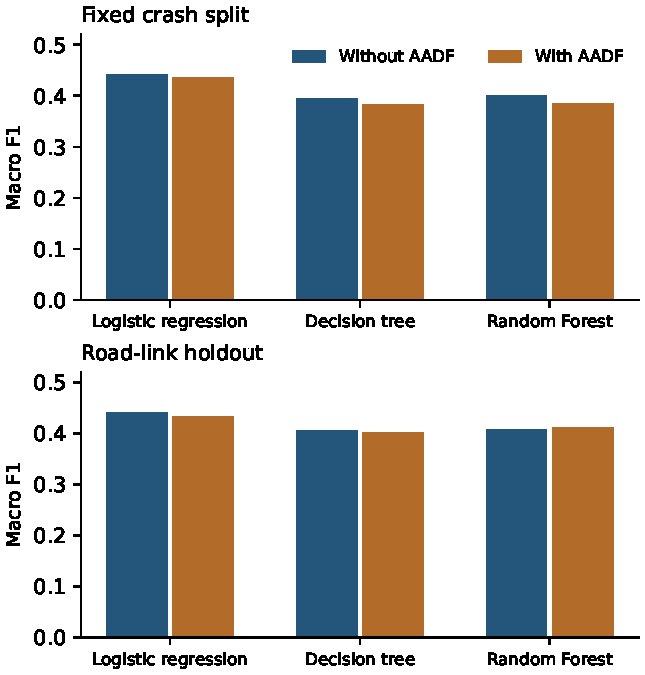
\includegraphics[width=\columnwidth]{results_plot.pdf}
\caption{Macro F1 by model and feature set under the two partition protocols. The road-link experiment retunes all families within its own development partitions.}
\label{fig:results}
\end{figure}

\section{Implementation and Reproducibility}
The repository provides source data attribution, prepared datasets, original notebooks, a standalone three-model runner, an unseen-link evaluator and six ready-to-load historical-split bundles. CSV inference validates required feature columns, binary vehicle flags and AADF values. A JSON interface translates named road, weather, surface and vehicle categories, a clock time and the posted speed limit into the prepared schema.

Nine automated tests cover partition integrity, leakage-column exclusion, score ordering, saved-model predictions, malformed scenarios and basic input validation. Continuous integration retrains the historical configurations and exercises both inference commands. Supplementary unseen-link metrics include partition sizes and zero link overlap. Data and software identifiers are retained in a reproducibility manifest. Model binaries use joblib and are intended to be loaded only from a trusted source.

\section{Limitations and Discussion}
Fatal cases remain scarce: one additional correct prediction changes fatal recall by about 2.04 percentage points on the crash-level test and 2.63 points on the link holdout. We do not claim statistical significance for small score differences or that one partition demonstrates universal superiority. Spatially adjacent links may still share conditions even when count-point identifiers are disjoint.

AADF is an annual-volume proxy covering selected major roads and is often estimated. It supplies neither congestion nor instantaneous vehicle density. A low score from this feature does not imply that well-timed live traffic measurements would be uninformative. Differences in crash reporting, geography, road types and severity definitions restrict transferability to other countries. No Indian dataset or future-year external test is evaluated here.

The models are observational and do not estimate causal effects of speed policy, weather or road changes. Output scores are not calibrated individual fatality risks. Their low fatal recall precludes claims of readiness for emergency dispatch or other safety-critical decisions. Further work should evaluate newer years, calibration and uncertainty, road-corridor grouping, ordinal models and richer exposure measurements using a prespecified evaluation protocol.

\section{Conclusion}
A reproducible severity classifier requires more than a high accuracy figure. Logistic regression leads macro F1 in the studied configurations, but detects only a minority of fatalities. AADF does not improve its macro F1 under either partition protocol, while the retuned forest shows a small gain on the unseen-link holdout. The completed workflow makes these trade-offs visible through fixed rows, explicit matching, separate model selection and test evaluation, reusable inference bundles and verified software checks.

\begin{thebibliography}{9}
\bibitem{chen} M.-M. Chen and M.-C. Chen, ``Modeling Road Accident Severity with Comparisons of Logistic Regression, Decision Tree and Random Forest,'' \emph{Information}, vol. 11, no. 5, art. 270, 2020, doi: 10.3390/info11050270.
\bibitem{fiorentini} N. Fiorentini and M. Losa, ``Handling Imbalanced Data in Road Crash Severity Prediction by Machine Learning Algorithms,'' \emph{Infrastructures}, vol. 5, no. 7, art. 61, 2020, doi: 10.3390/infrastructures5070061.
\bibitem{kim} S. Kim, Y. Lym and K.-J. Kim, ``Developing Crash Severity Model Handling Class Imbalance and Implementing Ordered Nature: Focusing on Elderly Drivers,'' \emph{Int. J. Environ. Res. Public Health}, vol. 18, no. 4, art. 1966, 2021, doi: 10.3390/ijerph18041966.
\bibitem{obasi} I. C. Obasi and C. Benson, ``Evaluating the effectiveness of machine learning techniques in forecasting the severity of traffic accidents,'' \emph{Heliyon}, vol. 9, no. 8, e18812, 2023, doi: 10.1016/j.heliyon.2023.e18812.
\bibitem{kuo} P.-F. Kuo, W.-T. Hsu, D. Lord and I G. B. Putra, ``Classification of autonomous vehicle crash severity: Solving the problems of imbalanced datasets and small sample size,'' \emph{Accident Analysis \& Prevention}, vol. 205, art. 107666, 2024, doi: 10.1016/j.aap.2024.107666.
\bibitem{dfttraffic} Department for Transport, ``Road traffic statistics downloads,'' AADF, count points and Major Roads Database, 2025 files. [Online]. Available: \url{https://roadtraffic.dft.gov.uk/downloads}
\bibitem{dftsafety} Department for Transport, ``Road safety open data,'' STATS19 collision and vehicle data and guide, 2025 files. [Online]. Available: \url{https://www.gov.uk/government/statistical-data-sets/road-safety-open-data}
\end{thebibliography}
\end{document}
